
\chapter{Numerical Validation}
\label{chp:NumMethodComp}

%use energy instead of hamiltonian

\section{Measuring Convergence and Conservation}
The numerical methods are assessed in this chapter by investigating their convergence and conservation properties. The convergence of these numerical methods is studied using analytic solutions to the governing equations and forced solutions to the forced Serre equations. While conservation is investigated by comparing the total of a conserved quantity in a numerical solution and comparing with the total of that quantity present in the initial conditions. We introduce notation for these measures and describe their calculation here, beginning with convergence.

\subsection{Measures of Convergence}
By measuring the relative difference between the numerical and analytic solutions as $\Delta x$ varies, the convergence of the numerical methods can be investigated. To measure the relative difference we use the $L_1$ vector norm; to compare the numerical and analytic solutions at the numerical grid locations $x_j$ at the end of the simulations. For a quantity $q$, the vector of its values $\vecn{q}$ at the grid locations $x_j$ and the corresponding numerical solution at those locations $\vecn{q^*}$; the $L_1$ norm is
\begin{equation}
L_1(\vecn{q},\vecn{q^*}) =  \left\lbrace \begin{array}{c r} 
\dfrac{||\vecn{q^*} - \vecn{q}||_{1}}{||\vecn{q}||_{1}} & ||\vecn{q}||_{1} > 0 \\ \\
{||\vecn{q^*}||_{1}} & ||\vecn{q}||_{1} = 0  \end{array}\right. . 
\label{eqn:L1qdef} 
\end{equation}


When no analytic solution is present, we can compare the distance between numerical solutions to gain some insight into how a sequence of numerical solutions are behaving. This allows us to demonstrate that a sequence of numerical solutions is convergent to some solution. To do this the $L_1$ vector norm is again used as in \eqref{eqn:L1qdef} except now both vectors are numerical solutions. Since both numerical solutions will have different grid locations, we only take the difference between the two at the common grid points. We have constructed our grids to accommodate for this, varying $\Delta x$ by successively dividing by $2$. This ensures that the grid locations generated by the larger $\Delta x$ value are all in the grid generated by the smaller $\Delta x$ value, and so we can compare both numerical solutions at the grid points generated by the larger $\Delta x$ value.  


\subsection{Measures of Conservation}
The conservation properties of the methods are established by calculating the total of a conserved quantity in the numerical solution $\mathcal{C}^*\left({\vecn{q^*}}\right)$ at the end of the simulation and comparing it to the total of that quantity for the initial conditions $\mathcal{C}\left({q(x,0)} \right)$, derived analytically. We do this again using the relative measure;
\begin{equation}
C_1(q,\vecn{q^*}) =  \left\lbrace \begin{array}{c r} 
\dfrac{|\mathcal{C}^*\left({\vecn{q^*}}\right) - \mathcal{C}\left({q(x,0)} \right)| }{|\mathcal{C}\left({q(x,0)} \right)|} & |\mathcal{C}\left({q(x,0)} \right)| > 0 \\ \\
|\mathcal{C}^*\left({\vecn{q^*}}\right)| & |\mathcal{C}\left({q(x,0)} \right)| = 0  \end{array}\right. . 
\label{eqn:C1qdef} 
\end{equation}
$\mathcal{C}^*\left({\vecn{q^*}}\right)$ was calculated using 3 point Gaussian quadrature over the $j^{th}$ cell and summing these cell integrals for all $j$. The three points needed to perform the Gaussian quadrature were calculated by interpolating the $j^{th}$ cell using a quartic that fits the nodal values $q_{j-2}$, $q_{j-1}$, $q_{j}$, $q_{j+1}$ and $q_{j+2}$. The Gaussian quadrature using three points is $5^{th}$ order accurate and interpolation by quartics is $5^{th}$ order accurate for the quantity $q$ and $4^{th}$ order accurate for its spatial derivative $\partial q /  \partial x$. Since all methods are third-order accurate or less, the error introduced by the calculation of $\mathcal{C}^*\left({\vecn{q^*}}\right)$ for the mass, momentum, $G$ and $\mathcal{H}$ will be dominated by the error introduced by the numerical solvers.

In some cases $\mathcal{C}\left({q(x,0)} \right)$ may be difficult to derive analytically. In this case we compare $\mathcal{C}^*\left(\vecn{q^*}\right)$ with $\mathcal{C}^*\left(\vecn{q}^0\right)$; where $\vecn{q}^0$ is the vector of the quantity at the grid locations used as the initial conditions of our numerical method. Comparing these we get 
\begin{equation}
C^*_1({\vecn{q}^0},\vecn{q^*}) =  \left\lbrace \begin{array}{c r} 
\dfrac{|\mathcal{C}^*\left({\vecn{q^*}}\right) - \mathcal{C}^*\left({\vecn{q}^0}\right)| }{|\mathcal{C}^*\left({\vecn{q}^0}\right)|} & |\mathcal{C}^*\left({\vecn{q}^0}\right)| > 0 \\ \\
|\mathcal{C}^*\left({\vecn{q^*}}\right)| & |\mathcal{C}^*\left({\vecn{q}^0}\right)| = 0  \end{array}\right. . 
\label{eqn:C*1qdef} 
\end{equation}


\section{Analytic Solution for Horizontal Bed}
To assess the ability of our numerical methods to solve the Serre equations with a horizontal bed \eqref{eqn:FullSerreConHorizBed} we use the solitary travelling wave solution \eqref{eqn:Solitondefhub} described in Chapter \ref{chp:Serreeqns}. This is a particular member of the family of periodic travelling wave solutions \cite{El-etal-2006}, but all these solutions except the trivial one provide a similar test for the numerical methods and so it is sufficient to only use the the solitary travelling wave solution.

For the solitary wave analytic solution all the terms in \eqref{eqn:FullSerreConHorizBed} must be adequately approximated by the numerical method to properly reproduce the analytic solution. Therefore this analytic solution serves as a very good benchmark for the ability of the numerical methods to accurately solve the Serre equations with a horizontal bed for smooth solutions.

For our numerical tests we used the solitary travelling wave solution we used \eqref{eqn:Solitondefhub} with $a_0 = 1m$ , $a_0 = 0.7m$ and $g= 9.81m/s^2$ at $t=0s$ as initial conditions in our numerical methods. The spatial domain was $[-250m,250m]$ and the problem was solved until $t= 50s$. This was done for a range of $\Delta x$ values that had the following form; $\Delta x = 100 / 2^k m$ with $k \in  \left[6,7, \dots,19\right]$. We satisfied the CFL condition with a CFL number of $Cr = 0.5$ by setting  $\Delta t = Cr / \sqrt{g\left(a_0 + a_1\right)}$. For $\text{FDVM}_2$ and $\text{FEVM}_2$ we used $\theta  = 1.2$ as the limiting parameter in the generalised minmod limiter \eqref{eqn:slopehGrecon}. 

The parameters $a_0 = 1m$ and $a_0 = 0.7m$ so that the non-linearity parameter $\epsilon = a_1 / a_0 = 0.7$ was large but beneath the breaking threshold for water waves []. Because $\epsilon$ is large the nonlinear effects are large and therefore so are the dispersive effects making this analytic solution a rigorous test of the numerical methods. For this spatial domain and a final time $t=50s$ there is no interaction of the wave and the boundary, therefore Dirichlet boundary conditions are appropriate.

\subsection{Results for Solitary Travelling Wave Solution}
%mention FEVM first?
An example numerical solution with $\Delta x = {100} / {2^{11}}m$ from all methods was plotted in Figure \ref{fig:SolitonExAll} against the analytic solution at $t= 50s$. We have only plotted an illustrative amount of the points in the numerical solution. From these plots it is clear that $\text{FDVM}_1$ performs significantly worse than the higher-order methods at reproducing the analytic solution, even for relatively fine grids where the wave is captured by more than $200$ cells. This is primarily due to the numerical diffusion introduced by the method, which has caused the wave in the numerical solution to decrease in amplitude and widen significantly. The higher-order numerical methods all accurately replicate the analytic solution, with insignificant differences in these plots due to the high resolution of the grid.

\begin{figure}
	\centering
	\begin{subfigure}{0.5\textwidth}
		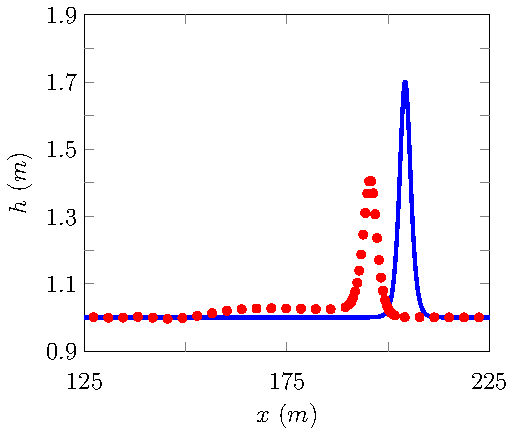
\includegraphics[width=\textwidth]{./chp5/figures/Analytic/Soliton/Example/FDVM1.pdf}
		\subcaption{$\text{FDVM}_1$}
		\vspace{0.5cm}
	\end{subfigure}%
	\begin{subfigure}{0.5\textwidth}
		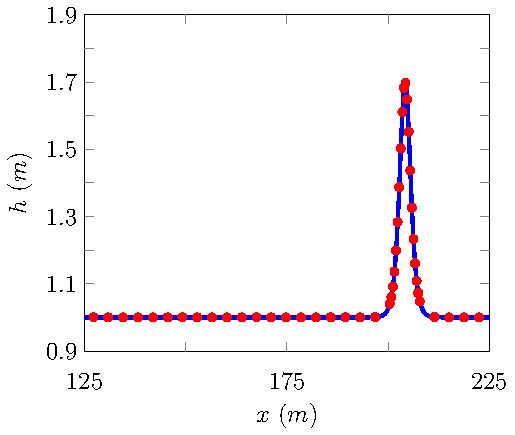
\includegraphics[width=\textwidth]{./chp5/figures/Analytic/Soliton/Example/FDVM2.pdf}
		\subcaption{$\text{FDVM}_2$}
		\vspace{0.5cm}
	\end{subfigure}
	\begin{subfigure}{0.5\textwidth}
		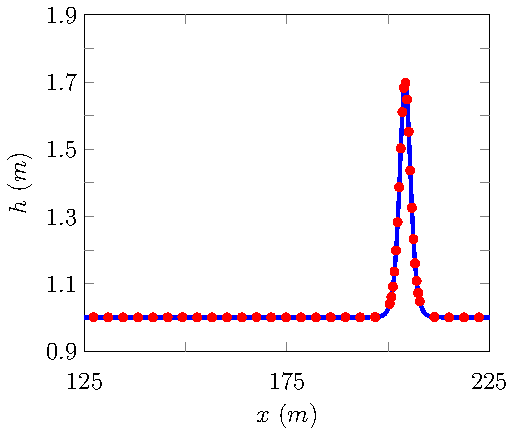
\includegraphics[width=\textwidth]{./chp5/figures/Analytic/Soliton/Example/FEVM2.pdf}
		\subcaption{$\text{FEVM}_2$}
		\vspace{0.5cm}
	\end{subfigure}%
	\begin{subfigure}{0.5\textwidth}
		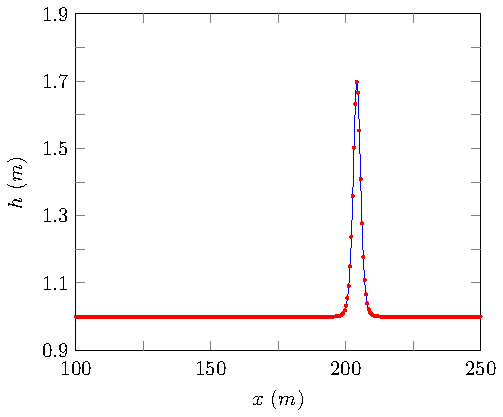
\includegraphics[width=\textwidth]{./chp5/figures/Analytic/Soliton/Example/FDVM3.pdf}
		\subcaption{$\text{FDVM}_3$}
		\vspace{0.5cm}
	\end{subfigure}
	\begin{subfigure}{0.5\textwidth}
		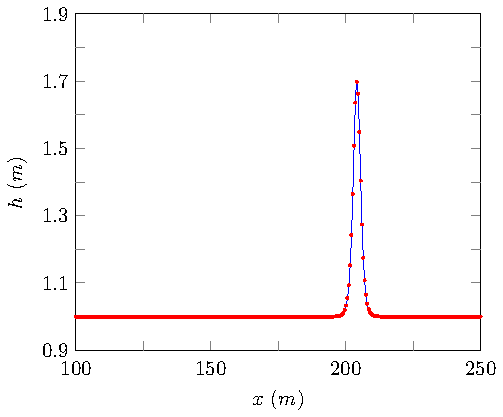
\includegraphics[width=\textwidth]{./chp5/figures/Analytic/Soliton/Example/D.pdf}
		\subcaption{$\mathcal{D}$}
		\vspace{0.5cm}
	\end{subfigure}%
	\begin{subfigure}{0.5\textwidth}
		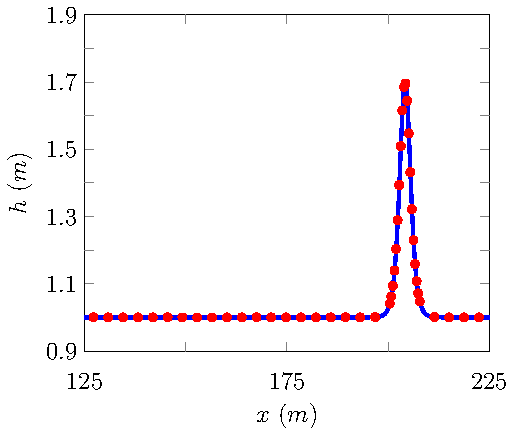
\includegraphics[width=\textwidth]{./chp5/figures/Analytic/Soliton/Example/W.pdf}
		\subcaption{$\mathcal{W}$}
		\vspace{0.5cm}
	\end{subfigure}
	\caption{Comparison of the analytic solution ({\color{blue} \solidrule}) and numerical solution with $\Delta x = {100} / {2^{11}}m$ ({\color{red} $\bullet$}) for the soliton problem at $t=50s$ for all methods.}
	\label{fig:SolitonExAll}
\end{figure}


The $L_1$ norm was calculated for $h$, $u$ and $G$ for all numerical solutions and was plotted against $\Delta x$ for all numerical methods in Figure \ref{fig:SolitonL1All}. From these plots it is clear that all numerical methods are convergent. The rate at which the numerical solutions converge to the analytic solution over $\Delta x$ is determined by the order of accuracy of the numerical scheme. All methods demonstrate the expected order of accuracy from the order of accuracy of the approximations used and their order of accuracy determined by linear analysis in Chapter \ref{chp:AnalNumMethod}.  

All methods more accurately reproduced the analytic solution for $h$ than either $G$ or $u$ across all $\Delta x$ values. This is due to the simplicity of the continuity equation \eqref{eqn:FullSerreConMass} compared to the irrotationality equation \eqref{eqn:Serreconsconmom} and the error in $u$ being dominated by the error in $G$. 

Increasing the order of accuracy of our numerical methods leads to smaller errors when comparing two methods for the same $\Delta x$ value, as Figure \ref{fig:SolitonL1All} clearly demonstrates. This is consistent with the example numerical solution in Figure \ref{fig:SolitonExAll}, where the lowest order accuracy scheme, $\text{FDVM}_1$ had the poorest reproduction of the analytic solution. However, even though the third-order accurate $\text{FDVM}_3$ is an improvement over its second-order counterparts, this improvement is less pronounced than the improvement between first and second-order methods.

%Difference between FEVM and W
For the second-order methods we find that $\text{FDVM}_2$ consistently produces the smallest $L_1$ error followed by $\text{FEVM}_2$, $\mathcal{W}$ and $\mathcal{D}$. The difference between the $\text{FDVM}_2$ and $\text{FEVM}_2$ is significant with errors of $\text{FEVM}_2$ being $2$ to $4$ times larger than $\text{FDVM}_2$. Both finite difference methods produce very similar errors which are about twice as large as the errors from $\text{FEVM}_2$. 

\begin{figure}
	\centering
	\begin{subfigure}{0.5\textwidth}
		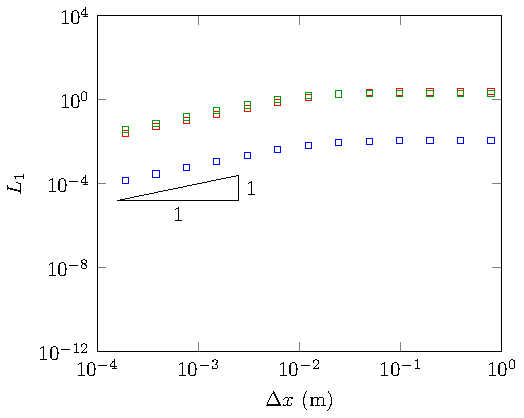
\includegraphics[width=\textwidth]{./chp5/figures/Analytic/Soliton/L1/FDVM1.pdf}
		\subcaption{$\text{FDVM}_1$}
		\vspace{0.5cm}
	\end{subfigure}%
	\begin{subfigure}{0.5\textwidth}
		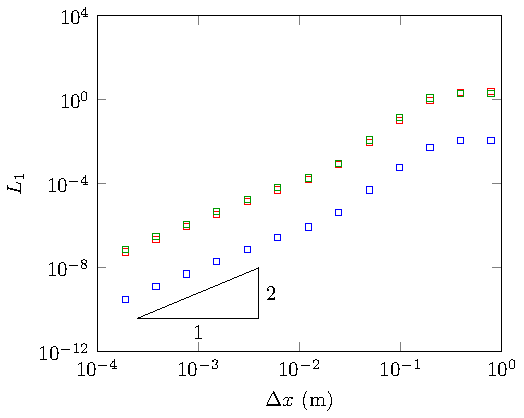
\includegraphics[width=\textwidth]{./chp5/figures/Analytic/Soliton/L1/FDVM2.pdf}
		\subcaption{$\text{FDVM}_2$}
		\vspace{0.5cm}
	\end{subfigure}
	\begin{subfigure}{0.5\textwidth}
		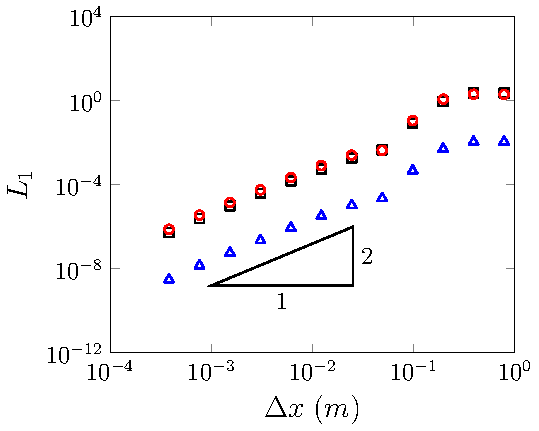
\includegraphics[width=\textwidth]{./chp5/figures/Analytic/Soliton/L1/FEVM2.pdf}
		\subcaption{$\text{FEVM}_2$}
		\vspace{0.5cm}
	\end{subfigure}%
	\begin{subfigure}{0.5\textwidth}
		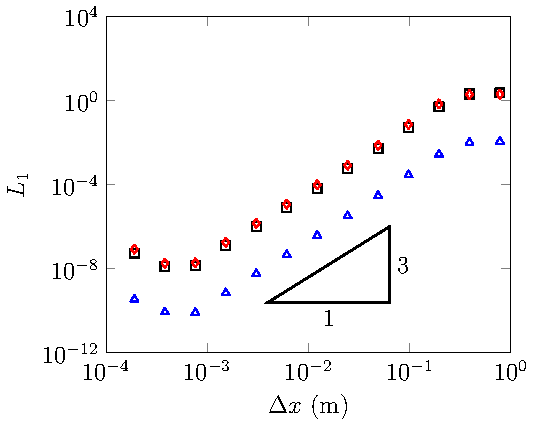
\includegraphics[width=\textwidth]{./chp5/figures/Analytic/Soliton/L1/FDVM3.pdf}
		\subcaption{$\text{FDVM}_3$}
		\vspace{0.5cm}
	\end{subfigure}
	\begin{subfigure}{0.5\textwidth}
		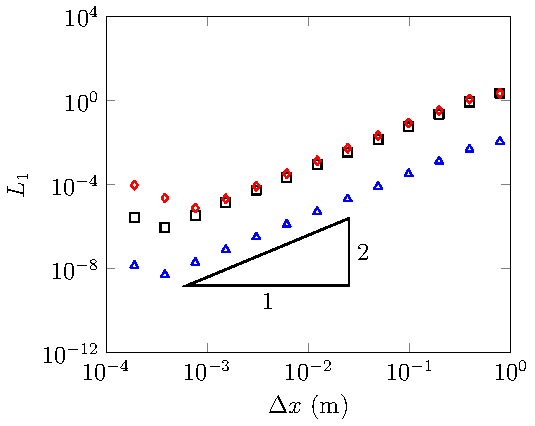
\includegraphics[width=\textwidth]{./chp5/figures/Analytic/Soliton/L1/D.pdf}
		\subcaption{$\mathcal{D}$}
		\vspace{0.5cm}
	\end{subfigure}%
	\begin{subfigure}{0.5\textwidth}
		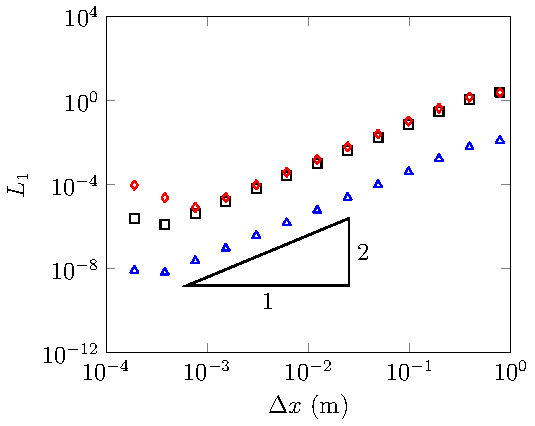
\includegraphics[width=\textwidth]{./chp5/figures/Analytic/Soliton/L1/W.pdf}
		\subcaption{$\mathcal{W}$}
		\vspace{0.5cm}
	\end{subfigure}
	\caption{Convergence plots as measured by the $L_1$ norm for $h$ (\trianglet{blue}), $u$ (\squaret{black}) and $G$ (\diamondt{red}) for the soliton problem for all methods.}
	\label{fig:SolitonL1All}
\end{figure}
%
%The $C_1$ norm was measured for mass ($h$), momentum ($uh$), $G$ and $\mathcal{H}$ using the analytic values [] and plotted in Figure \ref{fig:SolitonC1All}. From these plots it can be seen that all methods conserve mass at round-off error as long as $\Delta x$ is not too large, in this case requiring $\Delta x < 0.5m$. Since the FD methods perform just as well at conserving mass as the FDVM and FEVM, this suggests that using a finite volume method for the continuity equation \eqref{eqn:FullSerreConMass} is not necessary to conserve mass for this analytic solution. The $C_1$ norm suggests that $\text{FDVM}_3$ is the worst method for conservation of mass at lower $\Delta x$ values. However, this is due to the larger number of calculations required by this method leading to large accumulation of round-off errors, rather than a particular deficiency in $\text{FDVM}_3$ . 
%
%The conservation of momentum is significantly above round-off error, and for all numerical methods decreases at the rate determined by the order of accuracy or better. For the FDVM and the FEVM this is not surprising as $u$ is calculated from the elliptic equation, which will not necessarily conserve momentum in the system. While the FD methods which solve the momentum equation directly do not conserve momentum as finite difference methods are not necessarily conservative. Given the results for the $L_1$ norm, one might expect that the $C_1$ norm would decrease at the order of accuracy of the scheme. However, given that a quantity can be conserved and possess a large $L_1$ error, for instance translations of the solution, the fact that $C_1$ decreases faster than the order of accuracy is not surprising. 
%
%The second-order $\text{FEVM}_2$ performs the worst of all the methods for the conservation of momentum, even compared to the first-order $\text{FDVM}_1$. The superiority of the FDVM over the FEVM for conservation of momentum appears to be due to the use of the finite difference method to solve the elliptic equation, as both $\text{FDVM}_1$ and $\text{FDVM}_2$ use the same elliptic solver and both conserve momentum better than $\text{FEVM}_2$. 
%%momentum at point not an integral??
%
%For the conservation of $G$ we see that the case is very similar to the conservation of momentum, except for $\text{FEVM}_2$ which conserves $G$ at round-off error as long as $\Delta x$ isn't large. This implies that the FD used to solve the elliptic equation while resulting in smaller $L_1$ errors and better conservation of momentum, performs worse for the conservation of $G$. Therefore, we require a FEM to solve the elliptic equation so that our scheme conserves the conservative quantities $h$ and $G$. There appears to be some trade-off here between the conservation of $G$ and the conservation of momentum, with the $\text{FEVM}_2$ improving its conservation of $G$ by worsening its conservation of momentum. 
%
%The FD methods conserve $G$ better than they conserve momentum, this is surprising given that their governing partial differential equations are the conservation of mass and momentum equations \eqref{eqn:FullSerreNonCon}. 
%
%The conservation of the Hamiltonian decreases at the rate given by the order of accuracy of the method or better for all methods. Since no methods were designed using the conservation of Hamiltonian equation, its conservation is a good indication that these numerical method are appropriate for the Serre equations.
%
%Surprisingly the two FD methods conserve the Hamiltonian best, followed by $\text{FDVM}_2$, $\text{FEVM}_2$, $\text{FDVM}_3$ and $\text{FDVM}_1$.  All second-order methods conserve the Hamiltonian with an order of accuracy greater than $2$ while the first and third-order methods conserve the Hamiltonian at their respective order of accuracy. This suggests that even-order schemes have some advantage over odd-order schemes for the conservation of the Hamiltonian.
%
%\begin{figure}
%	\centering
%	\begin{subfigure}{0.5\textwidth}
%		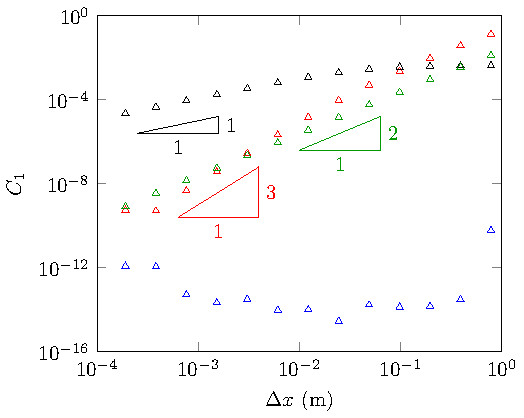
\includegraphics[width=\textwidth]{./chp5/figures/Analytic/Soliton/C1/FDVM1.pdf}
%		\subcaption{$\text{FDVM}_1$}
%		\vspace{0.5cm}
%	\end{subfigure}%
%	\begin{subfigure}{0.5\textwidth}
%		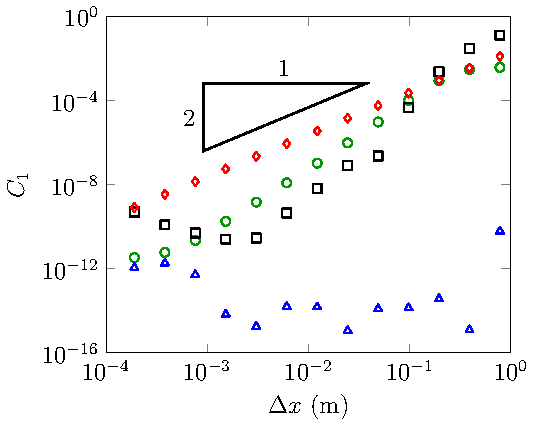
\includegraphics[width=\textwidth]{./chp5/figures/Analytic/Soliton/C1/FDVM2.pdf}
%		\subcaption{$\text{FDVM}_2$}
%		\vspace{0.5cm}
%	\end{subfigure}
%	\begin{subfigure}{0.5\textwidth}
%		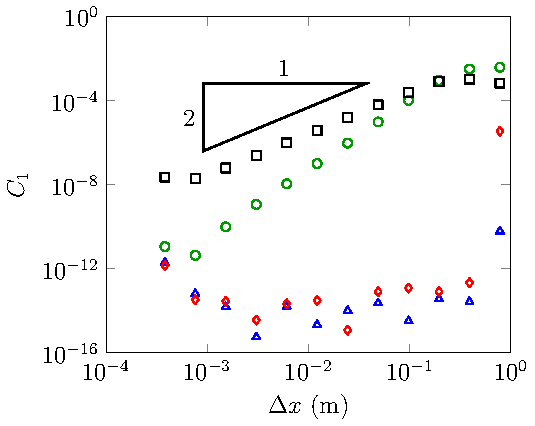
\includegraphics[width=\textwidth]{./chp5/figures/Analytic/Soliton/C1/FEVM2.pdf}
%		\subcaption{$\text{FEVM}_2$}
%		\vspace{0.5cm}
%	\end{subfigure}%
%	\begin{subfigure}{0.5\textwidth}
%		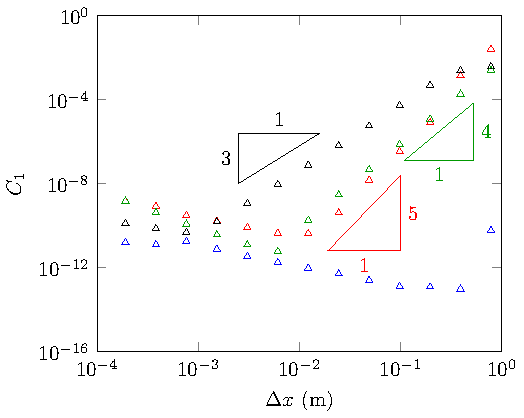
\includegraphics[width=\textwidth]{./chp5/figures/Analytic/Soliton/C1/FDVM3.pdf}
%		\subcaption{$\text{FDVM}_3$}
%		\vspace{0.5cm}
%	\end{subfigure}
%	\begin{subfigure}{0.5\textwidth}
%		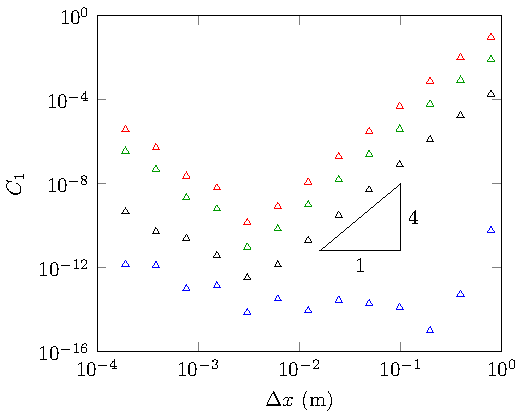
\includegraphics[width=\textwidth]{./chp5/figures/Analytic/Soliton/C1/D.pdf}
%		\subcaption{$\mathcal{D}$}
%		\vspace{0.5cm}
%	\end{subfigure}%
%	\begin{subfigure}{0.5\textwidth}
%		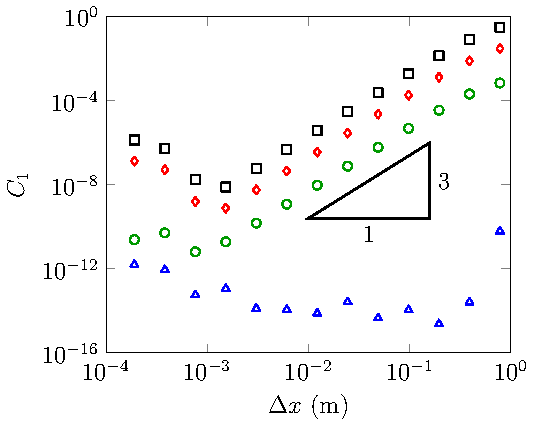
\includegraphics[width=\textwidth]{./chp5/figures/Analytic/Soliton/C1/W.pdf}
%		\subcaption{$\mathcal{W}$}
%		\vspace{0.5cm}
%	\end{subfigure}
%	\caption{Conservation plots as measured by $C_1$ for $h$ (\trianglet{blue}), $uh$ (\squaret{black}), $G$ (\diamondt{red}) and $\mathcal{H}$ (\circlet{green!60!black}) for the soliton problem for all methods.}
%	\label{fig:SolitonC1All}
%\end{figure}


\section{Analytic Solution for Variable Bathymetry}

To verify the validity of our numerical methods for the Serre equations with variable bathymetry \eqref{eqn:FullSerreNonCon} and assess the well balancing method employed we use the lake at rest analytic solution \eqref{eqn:LARdefhub}. 

The lake at rest solution \eqref{eqn:LARdefhub} associated with the bed profile
\begin{equation}
b(x) = a_1 \sin\left(a_2 x\right)
\end{equation}
was chosen to ensure that all terms with derivatives of the bed were tested. In particular the chosen parameters for our initial conditions of the numerical method were $a_0 = 0m$, $a_1 = 1m$ and $a_2 = 2 \pi / 50 $. This ensured that our lake at rest solution contained both wet and dry elements to demonstrate that the inclusion of both did not cause problems for the numerical method.

For the numerical solutions the spatial domain was $x \in \left[-112.5 m,87.5 m\right]$ and the final time was $t=10s$, with the standard gravitational acceleration $g= 9.81 m/s^2$. The spatial resolution of the method was varied like so $\Delta x = 100 / 2^k m$ with $k \in \left[4,17\right]$ and the CFL condition \eqref{eqn:CFLcond} was satisfied by having $\Delta t = Cr / \sqrt{g}$ with condition number $Cr = 0.5$. While the standard limiting parameter $\theta = 1.2$ was used for both the $\text{FEVM}_2$ and $\text{FDVM}_2$ in the generalised minmod limiter \eqref{eqn:slopehGrecon}. Dirichlet boundary conditions were used at both ends as the analytic solution is stationary. 

To assess the capability of the technique employed to achieve well balancing we compare two versions of the numerical methods $\text{FEVM}_2$ and $\text{FDVM}_2$; one with the well balancing and one without it. These are the only methods developed in this thesis that include variable bathymetry, allow dry beds and are well balanced and so these are the only numerical methods studied here.   

\subsection{Results for Lake at Rest}
Example numerical solutions with $\Delta x = 100/2^{10}$ at $t=10s$ for all versions of $\text{FEVM}_2$ and $\text{FDVM}_2$ are given in Figure \ref{fig:LakeAtRestEx}. The analytic solution and the numerical solution in these figures are indistinguishable at this scale, suggesting that both methods have recovered the analytic lake at rest solution.  

Closer examination of the $L_1$ errors depicted in Figure \ref{fig:LakeAtRestEL1} reveals a completely different picture for the two versions of each method. For both well balanced versions the errors in $h$ are consistently at round off level, while for both $G$ and $u$ the $L_1$ errors begin at round-off level and increases as $\Delta x$ decreases. The errors in $G$ and $u$ increase away from round-off due to accumulation of round of errors as the number of cells and time steps increases; thus creating an increase that is second-order. This accumulation of errors in $u$ and $G$ is a result of the finite difference methods employed in the source term approximation. 

Without well balancing the $\text{FEVM}_2$ and $\text{FDVM}_2$ lose second-order accuracy of $L_1$ error in $u$ and $G$ as the bed terms are not properly cancelled for the lake at rest stationary solution. The $L_1$ error in $h$ maintains the expected second-order convergence as the errors in $u$ and $G$ in this range of $\Delta x$ are too small to significantly contribute to the $L_1$ error of $h$ yet.

These results demonstrate the need for the well-balancing to be included in both numerical methods, as it is only with their inclusion that the lake at rest steady state can be accurately reproduced. 


%C1, H1 and L1

\begin{figure}
	\centering
	\begin{subfigure}{0.5\textwidth}
		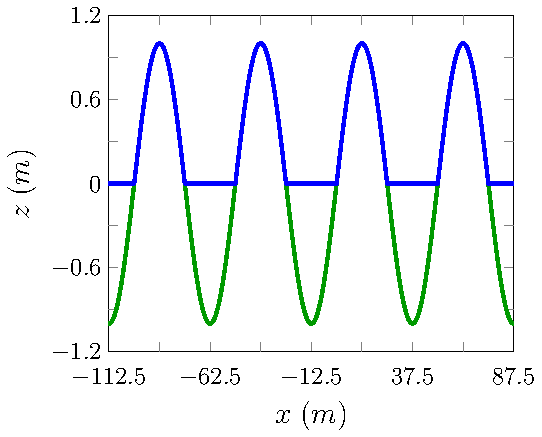
\includegraphics[width=\textwidth]{./chp5/figures/Analytic/LakeAtRest/Example/FEVMWB.pdf}
		\subcaption{$\text{FEVM}_2$ well balanced}
		\vspace{0.5cm}
	\end{subfigure}%
	\begin{subfigure}{0.5\textwidth}
		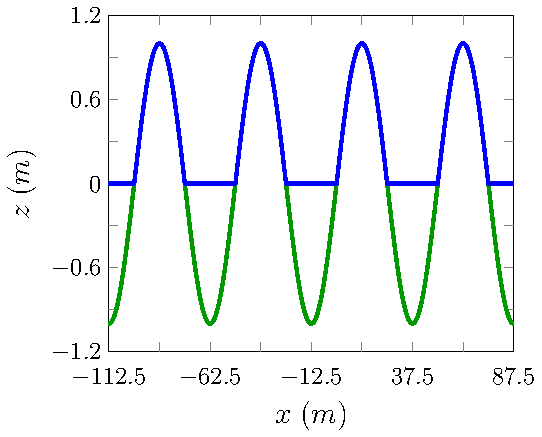
\includegraphics[width=\textwidth]{./chp5/figures/Analytic/LakeAtRest/Example/FEVMnWB.pdf}
		\subcaption{$\text{FEVM}_2$ not well balanced}
		\vspace{0.5cm}
	\end{subfigure}
	\begin{subfigure}{0.5\textwidth}
		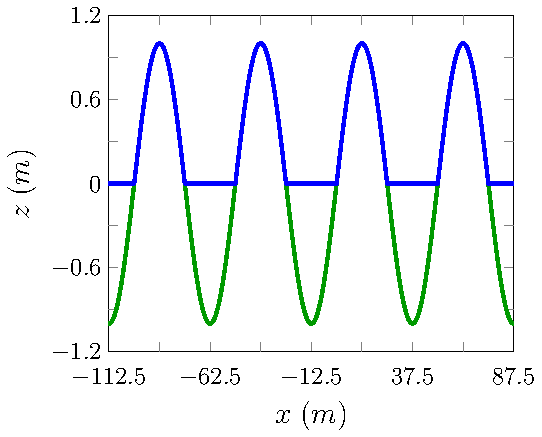
\includegraphics[width=\textwidth]{./chp5/figures/Analytic/LakeAtRest/Example/FDVMWB.pdf}
		\subcaption{$\text{FDVM}_2$ well balanced}
		\vspace{0.5cm}
	\end{subfigure}%
	\begin{subfigure}{0.5\textwidth}
		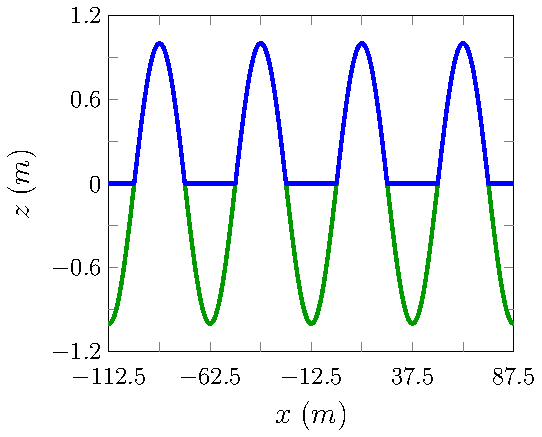
\includegraphics[width=\textwidth]{./chp5/figures/Analytic/LakeAtRest/Example/FDVMnWB.pdf}
		\subcaption{$\text{FDVM}_2$ not well balanced}
		\vspace{0.5cm}
	\end{subfigure}
	\caption{Comparison of the analytic solution ({\color{red} \solidrule}) and numerical solution with $\Delta x = {100} / {2^{10}}m$ ({\color{blue} \solidrule}) for the lake at rest problem at $t=10s$ for all methods.}
	\label{fig:LakeAtRestEx}
\end{figure}

\begin{figure}
	\centering
	\begin{subfigure}{0.5\textwidth}
		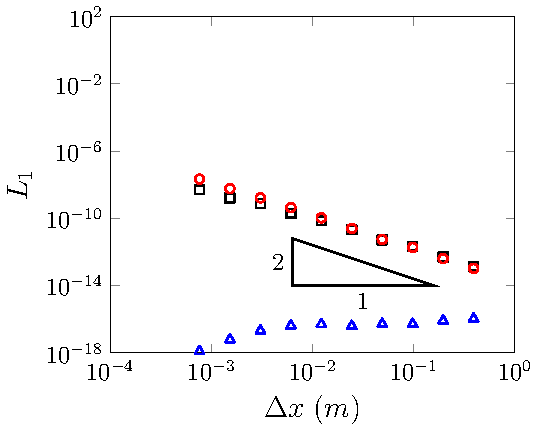
\includegraphics[width=\textwidth]{./chp5/figures/Analytic/LakeAtRest/L1/FEVMWB.pdf}
		\subcaption{$\text{FEVM}_2$ well balanced}
		\vspace{0.5cm}
	\end{subfigure}%
	\begin{subfigure}{0.5\textwidth}
		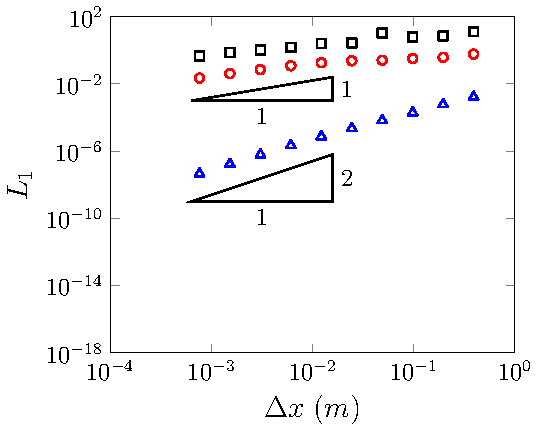
\includegraphics[width=\textwidth]{./chp5/figures/Analytic/LakeAtRest/L1/FEVMnWB.pdf}
		\subcaption{$\text{FEVM}_2$ not well balanced}
		\vspace{0.5cm}
	\end{subfigure}
	\begin{subfigure}{0.5\textwidth}
		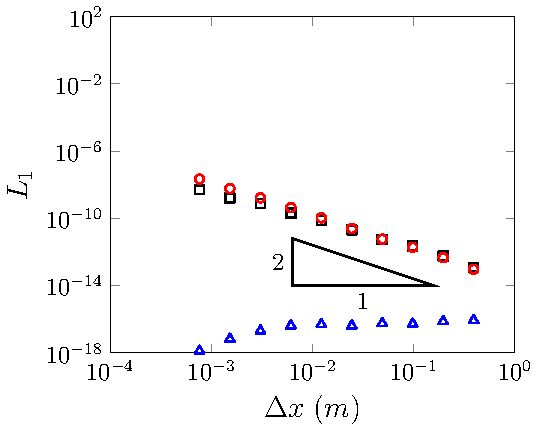
\includegraphics[width=\textwidth]{./chp5/figures/Analytic/LakeAtRest/L1/FDVMWB.pdf}
		\subcaption{$\text{FDVM}_2$ well balanced}
		\vspace{0.5cm}
	\end{subfigure}%
	\begin{subfigure}{0.5\textwidth}
		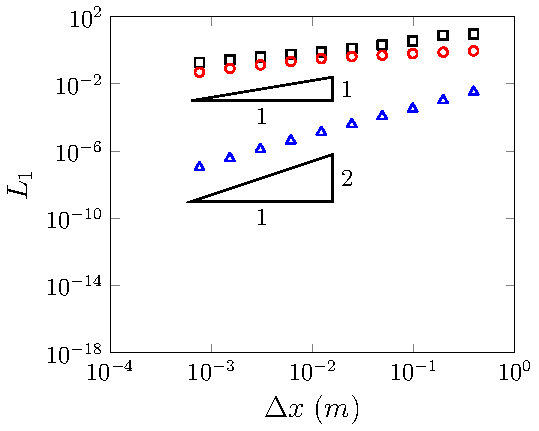
\includegraphics[width=\textwidth]{./chp5/figures/Analytic/LakeAtRest/L1/FDVMnWB.pdf}
		\subcaption{$\text{FDVM}_2$ not well balanced}
		\vspace{0.5cm}
	\end{subfigure}
	\caption{Convergence plots as measured by the $L_1$ norm for $h$ (\trianglet{blue}), $u$ (\squaret{black}) and $G$ (\diamondt{red}) for the lake at rest problem at $t=10s$ for all methods.}
	\label{fig:LakeAtRestEL1}
\end{figure}

%%\begin{figure}
%	\centering
%	\begin{subfigure}{0.5\textwidth}
%		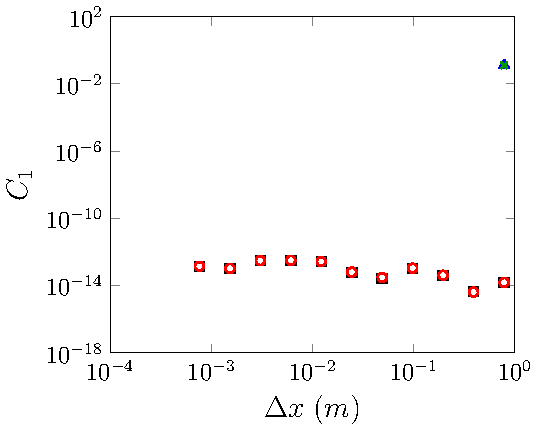
\includegraphics[width=\textwidth]{./chp5/figures/Analytic/LakeAtRest/C1/FEVMWB.pdf}
%		\subcaption{$\text{FEVM}_2$ well balanced}
%		\vspace{0.5cm}
%	\end{subfigure}%
%	\begin{subfigure}{0.5\textwidth}
%		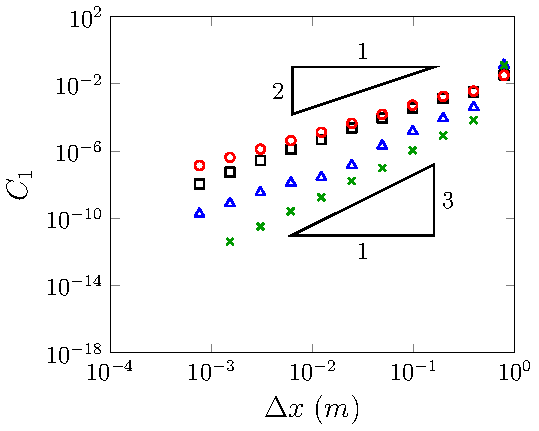
\includegraphics[width=\textwidth]{./chp5/figures/Analytic/LakeAtRest/C1/FEVMnWB.pdf}
%		\subcaption{$\text{FEVM}_2$ not well balanced}
%		\vspace{0.5cm}
%	\end{subfigure}
%	\caption{Convergence plots as measured by the $L_1$ norm for $h$ (\trianglet{blue}), $u$ (\squaret{black}) and $G$ (\diamondt{red}) for the lake at rest problem at $t=10s$ for all methods.}
%	\label{fig:LakeAtRestEC1}
%\end{figure}

\section{Forced Solutions}
%only L1
There are currently no known analytic solutions for the Serre equations that possess varying bathymetry and non-zero velocities. Therefore, the previous analytic solution comparisons do not provide a stringent test of all terms present in the Serre equations. To remedy this we use forced solutions which were introduced in Chapter \ref{chp:Serreeqns}. Since the source terms in the modified Serre equations \eqref{eqn:FullSerreConForced} can be determined and accounted for analytically, the only source of error in such numerical solutions are the numerical methods themselves and thus we should recover the theoretical second-order accuracy for $\text{FEVM}_2$ and $\text{FDVM}_2$. 

We performed validation tests for two forced solutions; one with a finite water depth everywhere and the other with a dry bed to validate both situations and to facilitate a comparison of the behaviour of our numerical solutions for both situations. To ensure that all terms of the Serre equations were accurately approximated in the numerical method the functions
\begin{subequations}
\begin{align}
\label{eqn:ForcedSolutionxt}
h^*(x,t) &= a_0 + a_1 \exp\left(-\dfrac{\left[\left(x - a_2 t\right) - a_3\right]^2}{2 a_4}\right), \\
u^*(x,t) &= a_5 \exp\left(-\dfrac{\left[\left(x - a_2 t\right) - a_3\right]^2}{2 a_4}\right), \\
b^*(x) &= a_6 \sin\left(a_7 x\right)
\end{align}
\end{subequations}
for the primitive variables were chosen, as for nontrivial choices of the parameters $a_i$ all terms in the Serre equations vary in space and time. 

Both validation studies used $a_1 = 0.5$, $a_2 = 2 \pi / \left(10 a_7\right)$, $a_3 = - 3\pi/ \left(2 a_7\right)$, $a_4 = \pi / 16 a_7$, $a_5 = 0.5$, $a_6 = 1.0$ and $a_7 = \pi / 25$ with $a_0= 1$ for the finite water depth forced solution and $a_0=0$ for the dry bed forced solution. 


\subsection{Results for Finite Water Depth} 
%a_0 = 1
For the finite water depth case $a_0 = 1m$ was chosen in equation \eqref{eqn:ForcedSolutionxt}. An example of the various quantities of the numerical solutions of  $\text{FEVM}_2$ and $\text{FDVM}_2$ for these forced solutions are given in Figures \ref{fig:ForcedWetFEVMP2PExAll} and \ref{fig:ForcedWetFDVMP2PExAll} for $\Delta x = $ [].

The numerical solutions of $\text{FEVM}_2$ and $\text{FDVM}_2$ with $\Delta x = $ [] and the forced solutions are identical for at these scales, reproducing the forced solution as it travels from peak to peak.

The $L_1$ error of $h$, $u$, $uh$ and $G$ for the $\text{FEVM}_2$ and $\text{FDVM}_2$ are given in Figure \ref{fig:L1convergenceforcedWet}. Both methods demonstrate the expected second-order accuracy. Since the source term of the modified Serre equations is added analytically and all terms must be accurately approximated by the methods for this forced solution, these results demonstrate that our scheme is completely second-order accurate for completely wet beds.

\begin{figure}
	\centering
	\begin{subfigure}{0.5\textwidth}
		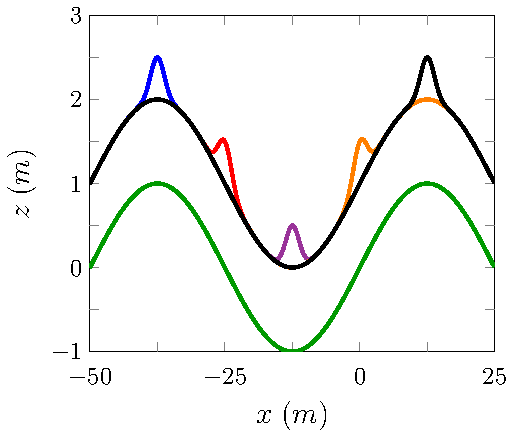
\includegraphics[width=\textwidth]{./chp5/figures/Forced/Wet/FEVMExw.pdf}
		\subcaption{$w$ and $b$ ({\color{green!60!black} \solidrule})}
		\vspace{0.5cm}
	\end{subfigure}%
	\begin{subfigure}{0.5\textwidth}
		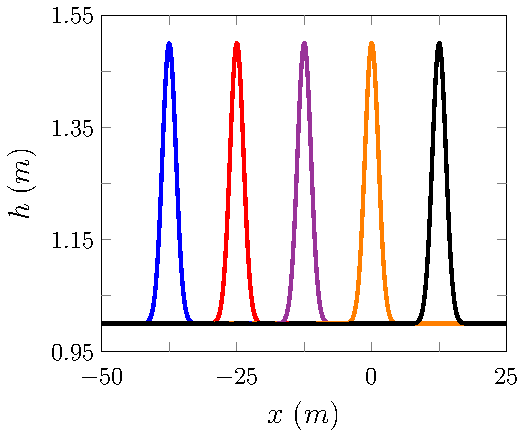
\includegraphics[width=\textwidth]{./chp5/figures/Forced/Wet/FEVMExh.pdf}
		\subcaption{$h$}
		\vspace{0.5cm}
	\end{subfigure}
	\begin{subfigure}{0.5\textwidth}
		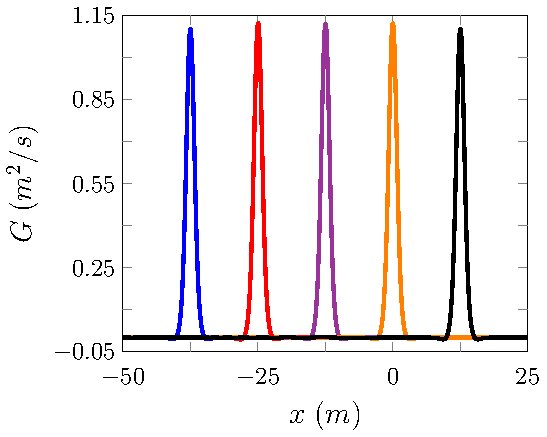
\includegraphics[width=\textwidth]{./chp5/figures/Forced/Wet/FEVMExG.pdf}
		\subcaption{$G$}
		\vspace{0.5cm}
	\end{subfigure}%
	\begin{subfigure}{0.5\textwidth}
		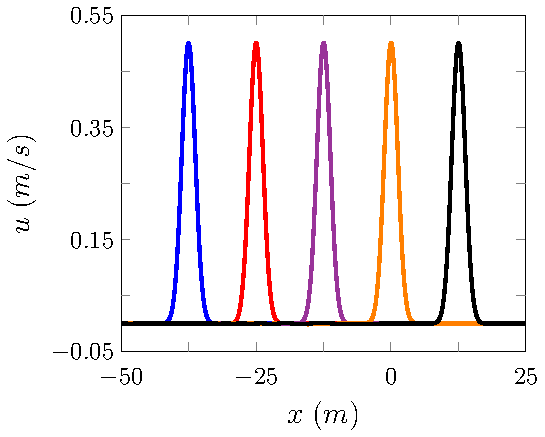
\includegraphics[width=\textwidth]{./chp5/figures/Forced/Wet/FEVMExu.pdf}
		\subcaption{$u$}
		\vspace{0.5cm}
	\end{subfigure}
	\caption{Plots of various quantities for the FEVM numerical solution at $0s$ ({\color{blue} \solidrule}), $2.5s$ ({\color{red} \solidrule}), $5.0s$ ({\color{violet!80!white} \solidrule}), $7.5s$ ({\color{orange} \solidrule}), $10.0s$ ({\color{black} \solidrule}) of the forced Serre equations.}
	\label{fig:ForcedWetFEVMP2PExAll}
\end{figure}

\begin{figure}
	\centering
	\begin{subfigure}{0.5\textwidth}
		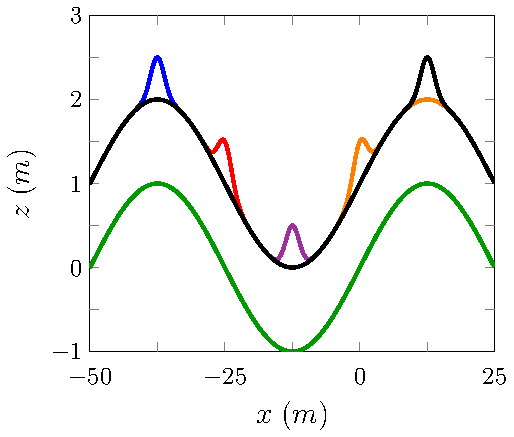
\includegraphics[width=\textwidth]{./chp5/figures/Forced/Wet/FDVMExw.pdf}
		\subcaption{$w$ and $b$ ({\color{green!60!black} \solidrule})}
		\vspace{0.5cm}
	\end{subfigure}%
	\begin{subfigure}{0.5\textwidth}
		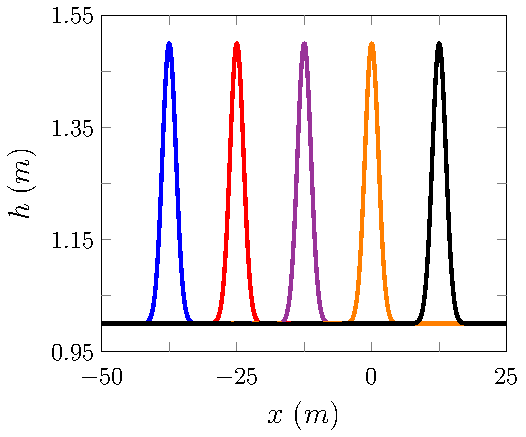
\includegraphics[width=\textwidth]{./chp5/figures/Forced/Wet/FDVMExh.pdf}
		\subcaption{$h$}
		\vspace{0.5cm}
	\end{subfigure}
	\begin{subfigure}{0.5\textwidth}
		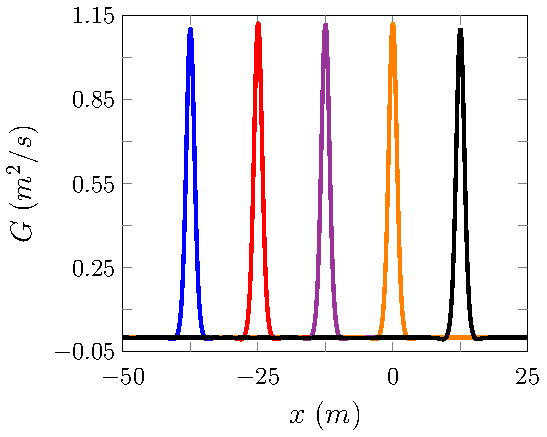
\includegraphics[width=\textwidth]{./chp5/figures/Forced/Wet/FDVMExG.pdf}
		\subcaption{$G$}
		\vspace{0.5cm}
	\end{subfigure}%
	\begin{subfigure}{0.5\textwidth}
		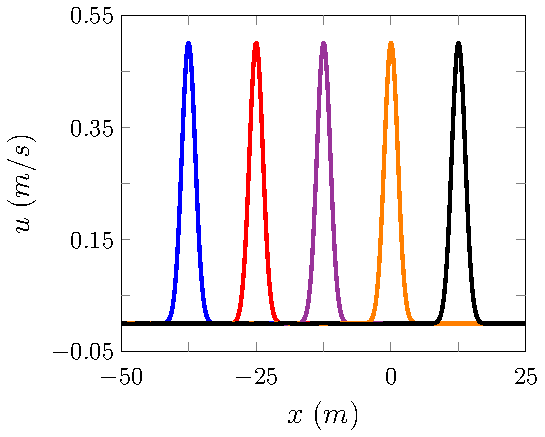
\includegraphics[width=\textwidth]{./chp5/figures/Forced/Wet/FDVMExu.pdf}
		\subcaption{$u$}
		\vspace{0.5cm}
	\end{subfigure}
	\caption{Plots of various quantities for the FDVM numerical solution at $0s$ ({\color{blue} \solidrule}), $2.5s$ ({\color{red} \solidrule}), $5.0s$ ({\color{violet!80!white} \solidrule}), $7.5s$ ({\color{orange} \solidrule}), $10.0s$ ({\color{black} \solidrule}) of the forced Serre equations.}
	\label{fig:ForcedWetFDVMP2PExAll}
\end{figure}


\begin{figure}
	\centering
	\begin{subfigure}{0.5\textwidth}
		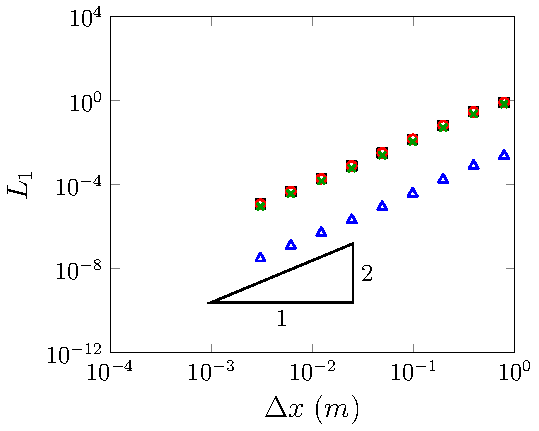
\includegraphics[width=\textwidth]{./chp5/figures/Forced/Wet/FEVML1.pdf}
		\subcaption{$\text{FEVM}_2$}
		\vspace{0.5cm}
	\end{subfigure}%
	%[]!!---!![]
	\begin{subfigure}{0.5\textwidth}
		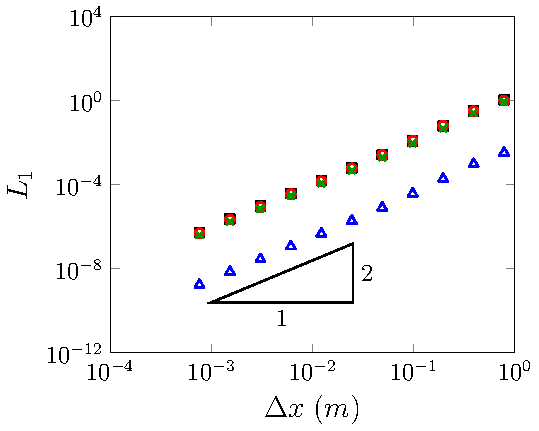
\includegraphics[width=\textwidth]{./chp5/figures/Forced/Wet/FDVML1.pdf}
		\subcaption{$\text{FDVM}_2$}
		\vspace{0.5cm}
	\end{subfigure}
	\caption{Convergence plots as measured by the $L_1$ norm for $h$ (\trianglet{blue}), $u$ (\squaret{black}),  $uh$ ({\color{green!60!black}$\times$})  and $G$ (\circlet{red}) for the forced solution problem for FEVM and FDVM at $t=10s$.}
	\label{fig:L1convergenceforcedWet}
\end{figure}


\subsection{Results with Dry Beds} 
%a_0 = 0
%mention the tolerance values
To demonstrate the capability of the methods to handle the wetting and drying of beds, we conducted a series of numerical simulations with \eqref{eqn:ForcedSolutionxt} where $a_0 = 0m$ for $\text{FEVM}_2$ and $\text{FDVM}_2$. 

An example numerical simulation demonstrating the evolution fo the wave is given in Figures \ref{fig:ForcedFEVMP2PExAll} and \ref{fig:ForcedFDVMP2PExAll} for $\text{FEVM}_2$ and $\text{FDVM}_2$ with $\Delta x = $[]. The methods both do very well at accurately reproducing the analytic solution for the stage $w$, $h$ and $G$. However, both fail to accurately reproduce $u$ as $h \rightarrow 0$, particularly behind the wave. 

%[explain why, also why its ok and expected]



The $L_1$ errors for both methods are given over the whole domain in Figure \ref{fig:ForcedSolDryL1}. Both methods are still displaying second-order convergence in all the quantities except $u$, as the large $u$ errors are only present for small $h$ and so are not captured by either $G$ or $uh$ for which $u$ is only ever multiplied by $h$, hiding the errors in $u$. Indeed if we restrict the domain to [] where $h$ is [] then we get that the convergence in $u$ is second-order as can be seen for both methods in Figure \ref{fig:ForcedSolDryL1restrict}.

Since the evolution of $h$ and $G$ only requires $u$ when it is multiplied by $h$, our result is a method that is second-order accurate for the conserved quantities even in the presence of dry beds.

Therefore this method can accurately handle the dry bed problem, although in such cases just studying the velocity will be misleading. 



\begin{figure}
	\centering
	\begin{subfigure}{0.5\textwidth}
		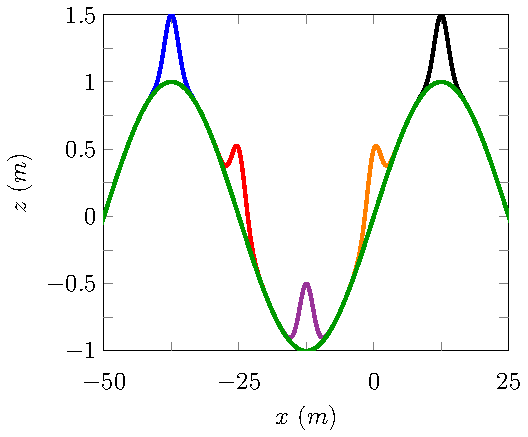
\includegraphics[width=\textwidth]{./chp5/figures/Forced/Dry/P2P/FEVMExw.pdf}
		\subcaption{$w$ and $b$ ({\color{green!60!black} \solidrule})}
		\vspace{0.5cm}
	\end{subfigure}%
	\begin{subfigure}{0.5\textwidth}
		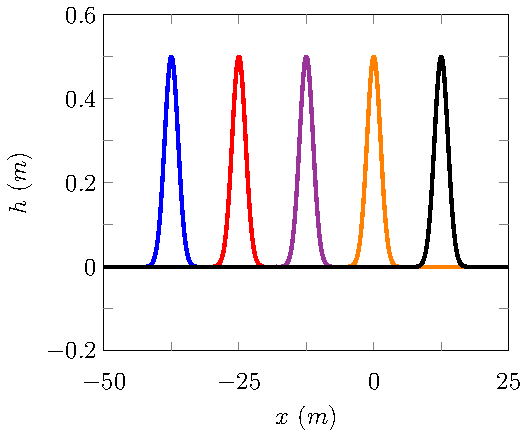
\includegraphics[width=\textwidth]{./chp5/figures/Forced/Dry/P2P/FEVMExh.pdf}
		\subcaption{$h$}
		\vspace{0.5cm}
	\end{subfigure}
	\begin{subfigure}{0.5\textwidth}
		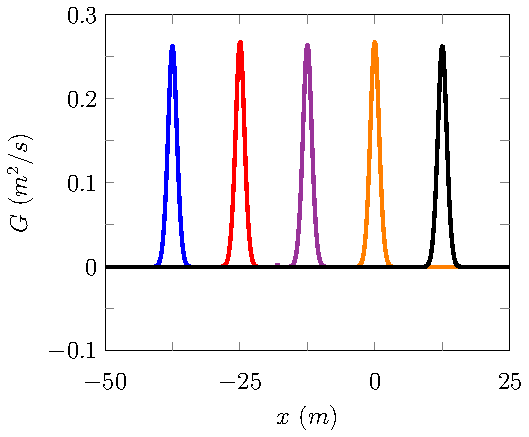
\includegraphics[width=\textwidth]{./chp5/figures/Forced/Dry/P2P/FEVMExG.pdf}
		\subcaption{$G$}
		\vspace{0.5cm}
	\end{subfigure}%
	\begin{subfigure}{0.5\textwidth}
		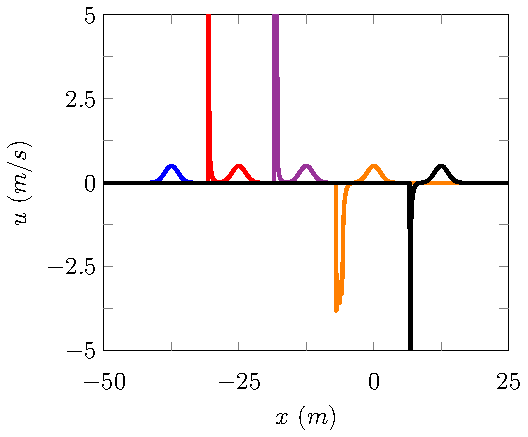
\includegraphics[width=\textwidth]{./chp5/figures/Forced/Dry/P2P/FEVMExu.pdf}
		\subcaption{$u$}
		\vspace{0.5cm}
	\end{subfigure}
	\caption{Plots of various quantities for the FEVM numerical solution at $0s$ ({\color{blue} \solidrule}), $2.5s$ ({\color{red} \solidrule}), $5.0s$ ({\color{violet!80!white} \solidrule}), $7.5s$ ({\color{orange} \solidrule}), $10.0s$ ({\color{black} \solidrule}) of the forced Serre equations.}
	\label{fig:ForcedFEVMP2PExAll}
\end{figure}

\begin{figure}
	\centering
	\begin{subfigure}{0.5\textwidth}
		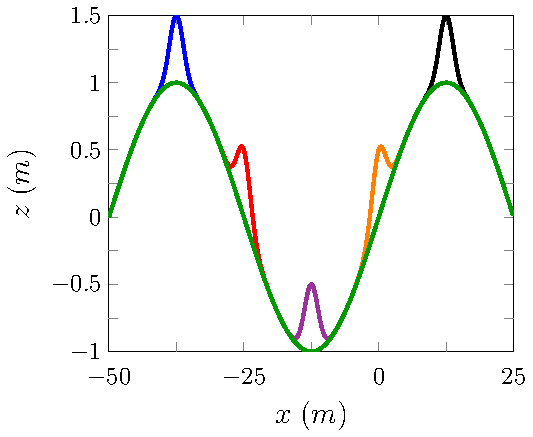
\includegraphics[width=\textwidth]{./chp5/figures/Forced/Dry/P2P/FDVMExw.pdf}
		\subcaption{$w$ and $b$ ({\color{green!60!black} \solidrule})}
		\vspace{0.5cm}
	\end{subfigure}%
	\begin{subfigure}{0.5\textwidth}
		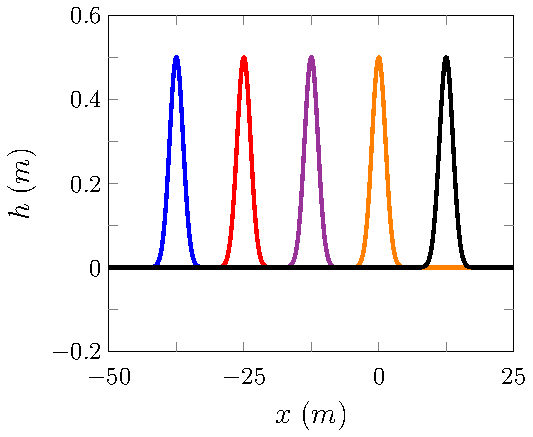
\includegraphics[width=\textwidth]{./chp5/figures/Forced/Dry/P2P/FDVMExh.pdf}
		\subcaption{$h$}
		\vspace{0.5cm}
	\end{subfigure}
	\begin{subfigure}{0.5\textwidth}
		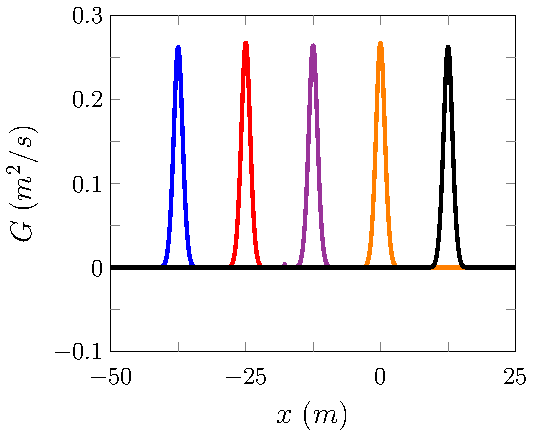
\includegraphics[width=\textwidth]{./chp5/figures/Forced/Dry/P2P/FDVMExG.pdf}
		\subcaption{$G$}
		\vspace{0.5cm}
	\end{subfigure}%
	\begin{subfigure}{0.5\textwidth}
		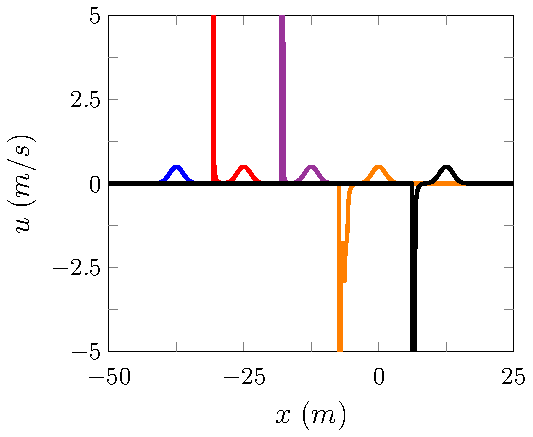
\includegraphics[width=\textwidth]{./chp5/figures/Forced/Dry/P2P/FDVMExu.pdf}
		\subcaption{$u$}
		\vspace{0.5cm}
	\end{subfigure}
	\caption{Plots of various quantities for the FDVM numerical solution at $0s$ ({\color{blue} \solidrule}), $2.5s$ ({\color{red} \solidrule}), $5.0s$ ({\color{violet!80!white} \solidrule}), $7.5s$ ({\color{orange} \solidrule}), $10.0s$ ({\color{black} \solidrule}) of the forced Serre equations.}
	\label{fig:ForcedFDVMP2PExAll}
\end{figure}


\begin{figure}
	\centering
	\begin{subfigure}{0.5\textwidth}
		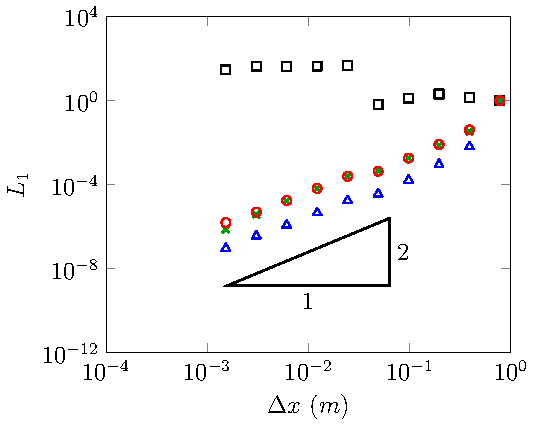
\includegraphics[width=\textwidth]{./chp5/figures/Forced/Dry/P2P/FEVML1.pdf}
		\subcaption{$\text{FEVM}_2$}
		\vspace{0.5cm}
	\end{subfigure}%
	%[]!!---!![]
	\begin{subfigure}{0.5\textwidth}
		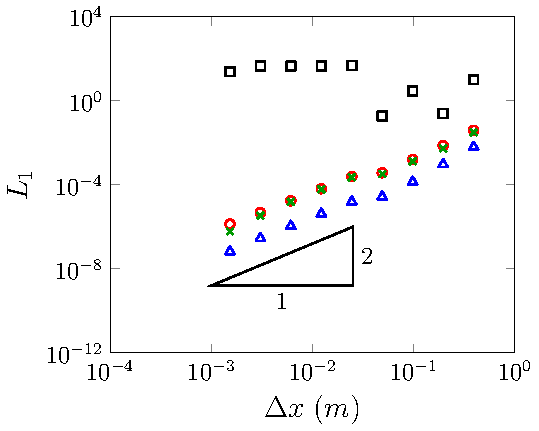
\includegraphics[width=\textwidth]{./chp5/figures/Forced/Dry/P2P/FDVML1.pdf}
		\subcaption{$\text{FDVM}_2$}
		\vspace{0.5cm}
	\end{subfigure}
	\caption{Convergence plots as measured by the $L_1$ norm for $h$ (\trianglet{blue}), $u$ (\squaret{black}),  $uh$ ({\color{green!60!black}$\times$})  and $G$ (\circlet{red}) for the forced solution problem for FEVM and FDVM at $t=10s$.}
	\label{fig:ForcedSolDryL1}
\end{figure}

\begin{figure}
	\centering
	\begin{subfigure}{0.5\textwidth}
		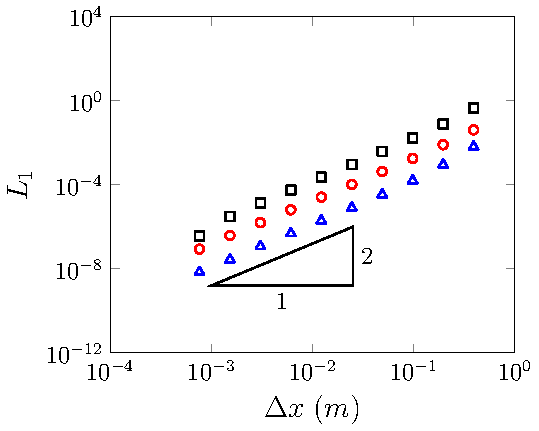
\includegraphics[width=\textwidth]{./chp5/figures/Forced/Dry/P2P/FEVML1red.pdf}
		\subcaption{$\text{FEVM}_2$}
		\vspace{0.5cm}
	\end{subfigure}%
	%[]!!---!![]
	\begin{subfigure}{0.5\textwidth}
		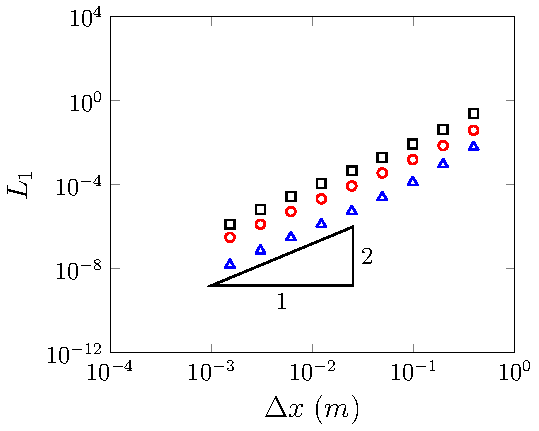
\includegraphics[width=\textwidth]{./chp5/figures/Forced/Dry/P2P/FDVML1red.pdf}
		\subcaption{$\text{FDVM}_2$}
		\vspace{0.5cm}
	\end{subfigure}
	\caption{Convergence plots as measured by the $L_1$ norm around the peak for $h$ (\trianglet{blue}), $u$ (\squaret{black}) and $G$ (\circlet{red}) for the forced solution problem for FEVM and FDVM at $t=10s$.}
	\label{fig:ForcedSolDryL1restrict}
\end{figure}
